% Sections 3.2 and 3.3: the two worked examples. Left: 5 models vote 3 placed, 2 not placed -> placed.
% Right: three regression models predict 6.2, 5.8, 7.0 LPA -> mean 6.33 LPA.
\documentclass[tikz,border=8pt]{standalone}
% Shared look for every TikZ diagram. Load with % Shared look for every TikZ diagram. Load with % Shared look for every TikZ diagram. Load with \input{../../tools/tikz-style.tex}
\usepackage[T1]{fontenc}
\usepackage{lmodern}
\renewcommand{\sfdefault}{lmr}  % diagrams use the same serif as the text
\usetikzlibrary{arrows.meta, positioning, shapes.geometric, calc, fit, backgrounds}
\definecolor{cblue}{HTML}{4C78A8}
\definecolor{corange}{HTML}{F58518}
\definecolor{cgreen}{HTML}{54A24B}
\definecolor{cred}{HTML}{E45756}
\definecolor{cpurple}{HTML}{B279A2}
\definecolor{cgrey}{HTML}{6B6B6B}
\tikzset{
  every picture/.style={font=\sffamily, line width=1.2pt},
  box/.style={draw=#1, fill=#1!12, rounded corners=4pt, align=center, inner sep=7pt, minimum height=1.1cm},
  box/.default=cgrey,
  arrow/.style={-{Stealth[length=3mm]}, draw=cgrey, line width=1.4pt},
  title/.style={font=\sffamily\bfseries\Large},
  note/.style={font=\sffamily\small, text=cgrey, align=center},
}
\AtBeginDocument{\hyphenpenalty=10000 \exhyphenpenalty=10000}

\usepackage[T1]{fontenc}
\usepackage{lmodern}
\renewcommand{\sfdefault}{lmr}  % diagrams use the same serif as the text
\usetikzlibrary{arrows.meta, positioning, shapes.geometric, calc, fit, backgrounds}
\definecolor{cblue}{HTML}{4C78A8}
\definecolor{corange}{HTML}{F58518}
\definecolor{cgreen}{HTML}{54A24B}
\definecolor{cred}{HTML}{E45756}
\definecolor{cpurple}{HTML}{B279A2}
\definecolor{cgrey}{HTML}{6B6B6B}
\tikzset{
  every picture/.style={font=\sffamily, line width=1.2pt},
  box/.style={draw=#1, fill=#1!12, rounded corners=4pt, align=center, inner sep=7pt, minimum height=1.1cm},
  box/.default=cgrey,
  arrow/.style={-{Stealth[length=3mm]}, draw=cgrey, line width=1.4pt},
  title/.style={font=\sffamily\bfseries\Large},
  note/.style={font=\sffamily\small, text=cgrey, align=center},
}
\AtBeginDocument{\hyphenpenalty=10000 \exhyphenpenalty=10000}

\usepackage[T1]{fontenc}
\usepackage{lmodern}
\renewcommand{\sfdefault}{lmr}  % diagrams use the same serif as the text
\usetikzlibrary{arrows.meta, positioning, shapes.geometric, calc, fit, backgrounds}
\definecolor{cblue}{HTML}{4C78A8}
\definecolor{corange}{HTML}{F58518}
\definecolor{cgreen}{HTML}{54A24B}
\definecolor{cred}{HTML}{E45756}
\definecolor{cpurple}{HTML}{B279A2}
\definecolor{cgrey}{HTML}{6B6B6B}
\tikzset{
  every picture/.style={font=\sffamily, line width=1.2pt},
  box/.style={draw=#1, fill=#1!12, rounded corners=4pt, align=center, inner sep=7pt, minimum height=1.1cm},
  box/.default=cgrey,
  arrow/.style={-{Stealth[length=3mm]}, draw=cgrey, line width=1.4pt},
  title/.style={font=\sffamily\bfseries\Large},
  note/.style={font=\sffamily\small, text=cgrey, align=center},
}
\AtBeginDocument{\hyphenpenalty=10000 \exhyphenpenalty=10000}

\begin{document}
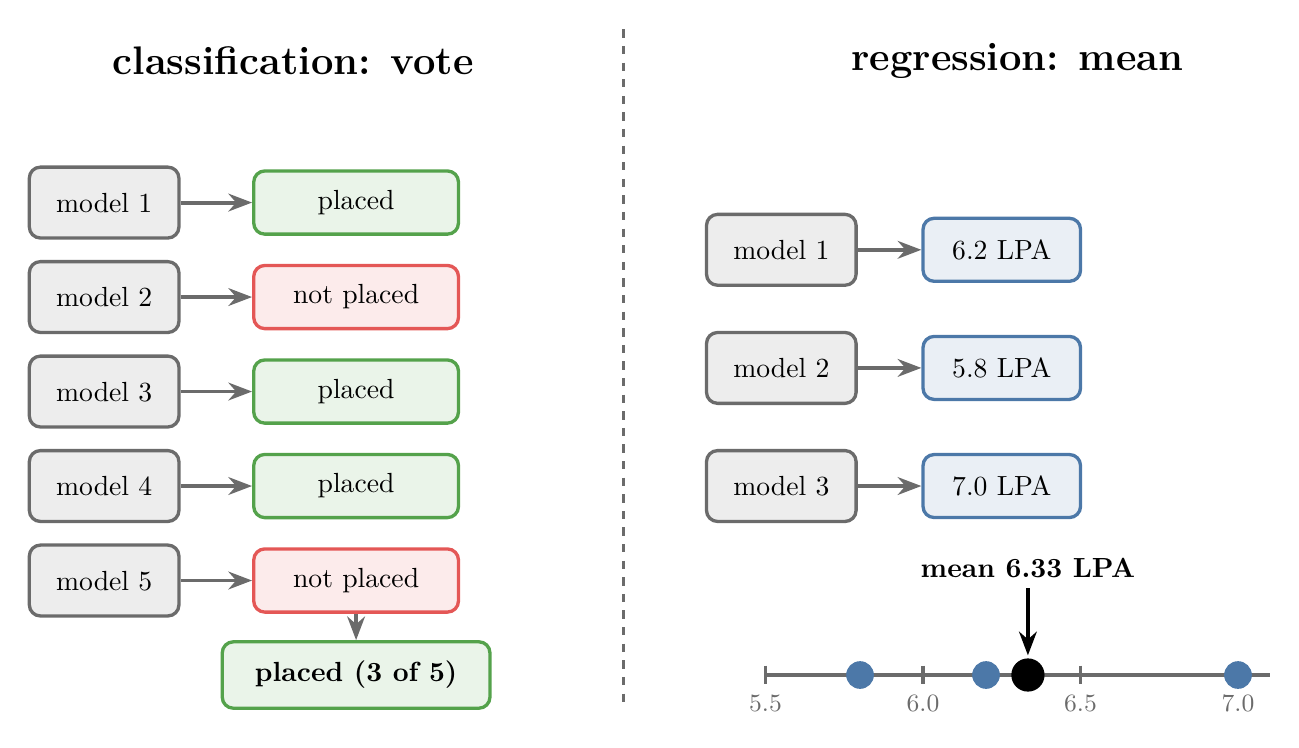
\begin{tikzpicture}[
  m/.style={box=cgrey, minimum width=1.9cm, minimum height=0.9cm},
  yes/.style={box=cgreen, minimum width=2.6cm, minimum height=0.8cm},
  no/.style={box=cred, minimum width=2.6cm, minimum height=0.8cm},
  num/.style={box=cblue, minimum width=2.0cm, minimum height=0.8cm}]
  % classification
  \node[title] at (2.4,1.2) {classification: vote};
  \foreach \i/\v/\w in {1/yes/placed,2/no/not placed,3/yes/placed,4/yes/placed,5/no/not placed} {
    \node[m] (m\i) at (0,-1.2*\i+0.6) {model \i};
    \node[\v] (v\i) at (3.2,-1.2*\i+0.6) {\w};
    \draw[arrow] (m\i) -- (v\i);
  }
  \node[yes, font=\sffamily\bfseries, minimum width=3.4cm] (out) at (3.2,-6.6) {placed (3 of 5)};
  \draw[arrow] (v5) -- (out);
  % regression
  \node[title] at (11.6,1.2) {regression: mean};
  \foreach \i/\v in {1/6.2,2/5.8,3/7.0} {
    \node[m] (r\i) at (8.6,-1.5*\i+0.3) {model \i};
    \node[num] (n\i) at (11.4,-1.5*\i+0.3) {\v{} LPA};
    \draw[arrow] (r\i) -- (n\i);
  }
  % number line
  \begin{scope}[shift={(8.4,-6.6)}]
    \draw[cgrey, line width=1.2pt] (0,0) -- (6.4,0);
    \foreach \x in {5.5,6.0,6.5,7.0} \draw[cgrey] ({(\x-5.5)*4},0.12) -- ({(\x-5.5)*4},-0.12) node[below, note] {\x};
    \foreach \x in {6.2,5.8,7.0} \fill[cblue] ({(\x-5.5)*4},0) circle (5pt);
    \fill[black] ({(6.333-5.5)*4},0) circle (6pt);
    \draw[arrow, draw=black] ({(6.333-5.5)*4},1.1) node[above, font=\sffamily\bfseries] {mean 6.33 LPA} -- ({(6.333-5.5)*4},0.25);
  \end{scope}
  \draw[cgrey, dashed] (6.6,1.6) -- (6.6,-7);
\end{tikzpicture}
\end{document}
